\section{Hyperbolic geometry}

It is the goal of this section to introduce a general method for the construction of fundamental regions with respect to the action of $\PSL{\Z}$ and its subgroups on $\EU$ which relies on the concepts of 2-dimensional hyperbolic geometry. 

\index{Hyperbolic!geometry}
Plane (\ie 2-dimensional) hyperbolic geometry is obtained from 2-di\-men\-si\-o\-nal Euclidean geometry by replacing the parallel postulate by the following axiom: 
\begin{enumerate}[(A)]
\item
\emph{Let $X$ be a point and $L$ be a line on the (hyperbolic) plane, such that $L$ does not pass through $X$. Then there is more than one line $L^\prime$ passing through $X$ which does not meet $L$.}
\end{enumerate}

There are various mathematical models of hyperbolic geometry. We will use a model based on the notions of generalized disks and generalized circles which we introduced in Section~\ref{sec_GenCircles}.

\begin{definition}[Elements of hyperbolic geometry]
\label{def_HypGeomModel}
\index{Proper point}
\index{Improper point}
\index{Hyperbolic!line}
\index{Hyperbolic!plane}
\index{H-line}
\index{H-plane}
\index{Horizon}
Let $\mathcal{P} \subseteq \C$ be a generalized disk, which serves as a model for 2-dimensional hyperbolic geometry. In this context, we will refer to $\mathcal{P}$ as \emph{hyperbolic plane} (for short \emph{h-plane}). The interior points of $\mathcal{P}$ are called \emph{proper points}; the boundary points of $\mathcal{P}$ are called \emph{improper points}. The set of all improper points (which is a generalized circle) is called the \emph{horizon} of $\mathcal{P}$.\footnote{The notions of proper and improper points as well as horizon are taken over from \Fenchel{}.} Every generalized circle $C$, which intersects the horizon of $\mathcal{P}$ orthogonally in two distinct (improper) points, gives rise to exactly one \emph{hyperbolic line} (for short \emph{h-line}) $L$ which is given by $L = C \cap \mathcal{P}$. 
\end{definition}

In the above model of hyperbolic geometry, the angular measure is taken over from Euclidean geometry, \ie the angle enclosed by two h-lines which intersect each other in a proper point $z \in \mathcal{P}$ is defined as the Euclidean angle enclosed by the (Euclidean) tangents of the h-lines at the point $z$. It now remains to introduce a measure for the distance between proper points in $\mathcal{P}$.

\begin{definition}[Metric]
\index{Metric}
Let $\mathcal{S}$ be nonempty a set. A function $d : \mathcal{S} \times \mathcal{S} \to \R$ is a \emph{metric} on $\mathcal{S}$, if the following conditions are satisfied for all $x,y,z \in \mathcal{S}$:
\begin{enumerate}[(i)]
\item \label{itm_MetricNonneg}
\emph{Non-negativity:} $d(x,y) \ge 0$.
\item \label{itm_MetricCoincidence}
\emph{Coincidence axiom:} $d(x,y) = 0$ if and only if $x = y$.
\item \label{itm_MetricSymmetry}
\emph{Symmetry:} $d(x,y) = d(y,x)$.
\item \label{itm_MetricTriIneq}
\emph{Triangle inequality:} $d(x,z) \le d(x,y) + d(y,z)$.
\end{enumerate}
\end{definition}
\begin{remark} From
\begin{equation*}
0 = d(x,x) \le d(x,y) + d(y,x) = 2 d(x,y),
\end{equation*}
we see that non-negativity (\ref{itm_MetricNonneg}) is implied by the conditions (\ref{itm_MetricCoincidence}), (\ref{itm_MetricSymmetry}) and (\ref{itm_MetricTriIneq}).
\end{remark}

\begin{definition}[Isometry]
\label{dfn_IsometryRigidMotion}
\index{Isometry}
Let $\mathcal{S}$ be a set and $d$ be a metric on $\mathcal{S}$. A map $\phi : \mathcal{S} \to \mathcal{S}$ is called an \emph{isometry}, if it leaves distances invariant, \ie if
\begin{equation*}
d(x,y) = d(\phi(x), \phi(y)) \quad \text{for all } x,y \in \mathcal{S}.
\end{equation*}
\end{definition}

\begin{remark}
It is direct to see that the set of all bijective isometries forms a group under the operation of function composition. Note that the coincidence axiom (\ref{itm_MetricCoincidence}) implies that isometries are necessarily injective. However, in general they do not need to be surjective.
\end{remark}

\index{Rigid motion}
We wish to introduce a metric on the h-plane $\mathcal{P}$, such that every M�bius transformation which maps $\mathcal{P}$ onto itself is an isometry of $\mathcal{P}$. Clearly all M�bius transformations with this property form a group. We will refer to the transformations of this group as \emph{rigid motions}\footnote{A rigid motion is an isometry which additionally leaves angles and their orientation invariant.} of the h-plane. 

\index{Cross ratio}
For the definition of such a metric we will take advantage of the so-called \emph{cross ratio}. Note that in literature for the term ``cross ratio'' different notations and definitions are used. We will adhere to \Caratheodory{} in this regard whose derivation of the cross ratio's elementary properties is particularly concise and elegant.

\begin{definition}
\label{dfn_CrossRatio}
Let $z_1,z_2,z_3,z_4 \in \EC$ be numbers of the extended complex plane with the restriction that at most two of these numbers are equal. The \emph{cross-ratio} $(z_1,z_2,z_3,z_4) \in \EC$ is defined as
\begin{equation}
\label{eqn_CrossRatio}
(z_1,z_2,z_3,z_4) := \crossrat{z_1}{z_2}{z_3}{z_4}.
\end{equation}
Note that in the case of an infinite quantity $z_k = \infty$, the cross ratio  shall be evaluated by formally dividing the two respective factors in the numerator and denominator of (\ref{eqn_CrossRatio}) by $z_k$ and by substitution of expressions $\reci{\infty}$ with zero.
\end{definition}

We will need the following important properties of the cross ratio:

\begin{lemma}[Invariance under M�bius transformations]
\label{lem_CrossRatioInvariance}
Let $\phi \in \PGL{\C}$ be a M�bius transformation and $z_1,z_2,z_3,z_4 \in \EC$ such that their cross ratio is defined. Set $w_j := \phi(z_j)$ for $j \in \{1,2,3,4\}$. The cross ratios of the numbers $z_j$ and $w_j$ are equal, \ie
\begin{equation}
\label{eqn_CrossRatioInvariance}
(z_1,z_2,z_3,z_4) = (w_1,w_2,w_3,w_4).
\end{equation}
\end{lemma}
\begin{proof}
Let us write the M�bius transformation $\phi$ as $\phi(z) = \moebius{a}{b}{c}{d}{z}$. For $i,j \in \{1,2,3,4\}$, we have
\begin{equation*}
w_i - w_j 
= \moebius{a}{b}{c}{d}{z_i} - \moebius{a}{b}{c}{d}{z_j} 
= \frac{ad - bc}{(c z_i + d)(c z_j + d)} \cdot (z_i - z_j).
\end{equation*}
Consequently, if we define
\begin{equation*}
A := \frac{(ad - bc)^2}{(c z_1 + d)(c z_2 + d)(c z_3 + d)(c z_4 + d)},
\end{equation*}
we obtain
\begin{equation*}
(w_1 - w_2)(w_3 - w_4) = A(z_1 - z_2)(z_3 - z_4).
\end{equation*}
On the other hand, exploiting the symmetry of $A$ with respect to the numbers $z_j$, we have
\begin{equation*}
(w_1 - w_3)(w_2 - w_4) = A(z_1 - z_3)(z_2 - z_4).
\end{equation*}
In the case when all involved numbers $z_j$ and $w_j$ are finite (and in particular $A$ is finite and nonzero), division of these two equations yields (\ref{eqn_CrossRatioInvariance}). The prove of the general case, when one or two of the numbers $z_j$ (\resp $w_j$) are $\infty$, involves some inconvenient case distinctions which we will not carry out here.
\end{proof}

\begin{lemma}
\label{lem_CrossRatioMoebius}
Let $z_1, z_2, z_3 \in \EC$ be pairwise distinct. The function
\begin{equation}
\label{eqn_CrossRatioMoebius}
\fundef{\lambda}{\EC}{\EC}{z}{(z_1,z_2,z_3,z)}
\end{equation}
is a M�bius transformation and satisfies $\lambda(z_1) = 1$, $\lambda(z_2) = \infty$, $\lambda(z_3) = 0$.
\end{lemma}
\begin{proof}
In the case when $\infty \notin \{z_1,z_2,z_3\}$, by setting $a := z_2 - z_1$, $b := z_2 (z_1 - z_2)$, $c := z_3 - z_1$ and $d := z_2 (z_1 - z_3)$ we can obviously write 
\begin{equation*}
\lambda(z) = \crossrat{z_1}{z_2}{z_3}{z} = \moebius{a}{b}{c}{d}{z}.
\end{equation*}
Moreover, we have
\begin{equation*}
ad - bc = (z_1 - z_2)(z_2 - z_3)(z_3 - z_1).
\end{equation*}
By assumption the numbers $z_j$ are pairwise distinct and therefore $\lambda$ is indeed a M�bius transformation. Note that for the other case, when some $z_k = \infty$, the cross ratio needs to be evaluated as specified in Definition~\ref{dfn_CrossRatio} and the coefficients $a,b,c,d$ need to be adapted appropriately. The statement on the images of $z_1,z_2,z_3$ under $\lambda$ is readily verified.
\end{proof}

\begin{corollary}
\label{cor_CrossRatioGCircle}
Denoting the extended real axis by $\R_\infty := \R \cup \{\infty\}$, the map $\lambda : \EC \to \EC$ from (\ref{eqn_CrossRatioMoebius}) satisfies $\lambda(z) \in \R_\infty$ if and only if $z$ lies on the generalized circle which is determined by the points $z_1,z_2,z_3$.
\end{corollary}
\begin{proof}
This statement is a consequence of the fact that $\lambda$ is a M�bius transformation and therefore maps the g-circle determined by the points $z_1,z_2,z_3$ pointwise one-to-one to the extended real axis $\R_\infty$.
\end{proof}

The above properties of the cross ratio allow to define a metric on the hyperbolic plane $\mathcal{P}$ the following way:

\begin{definition}[\Poincare{} metric]
\label{dfn_PoincareMetric}
\index{Poincar{\'e}!metric}
\index{Hyperbolic!distance}
Let $z_1, z_2 \in \mathcal{P}$ be two distinct proper points of the hyperbolic plane and let $L$ be the unique h-line joining $z_1$ with $z_2$. Label the two (improper) endpoints of $L$ by $\infty_1$ and $\infty_2$, such that $\infty_1, z_1, z_2, \infty_2$ are in order along the h-line $L$. The hyperbolic distance between $z_1$ and $z_2$ is defined as
\begin{equation}
\label{eqn_PoincareMetric}
\hypdist{z_1}{z_2} := \reci{2} \log \chi \quad \text{with } \chi := (z_1,\infty_2,\infty_1,z_2).
\end{equation}
Additionally we define $\hypdist{z}{z} = 0$ for all proper points $z \in \mathcal{P}$.
\end{definition}

\begin{theorem}
The hyperbolic distance defined in $(\ref{eqn_PoincareMetric})$ is a metric on the hyperbolic plane $\mathcal{P}$ which we call the \emph{\Poincare{} metric} on $\mathcal{P}$.
\end{theorem}
\begin{proof}[Sketch of proof]
The cross ratio $\chi$ in (\ref{eqn_PoincareMetric}) may alternatively be written as $\chi = \lambda(z_2)$, where $\lambda(z) := (z_1,\infty_2,\infty_1,z)$ is, according to Lemma~\ref{lem_CrossRatioMoebius}, a M�bius transformation satisfying $\lambda(z_1) = 1$ and $\lambda(\infty_2) = \infty$. Corollary~\ref{cor_CrossRatioGCircle} ensures that $\lambda(z)$ is real for all $z$ lying on the h-line $L$. Since $\lambda$ is a continuous map, it follows that $\lambda$ maps the h-line segment $S \subseteq L$ which is bounded by the points $z_1$ and $\infty_2$ pointwise one-to-one to the interval $[1,\infty] \subseteq \R_\infty$. For this reason, the hyperbolic metric is non-negative and $\hypdist{z_1}{z_2} \to 0$ as $z_2$ approaches $z_1$ along $S$. Similarly, $\hypdist{z_1}{z_2} \to \infty$ as $z_2$ approaches $\infty_2$ along $S$.

The symmetry of $d_\text{hyp}$ can easily be verified: Note that exchanging $z_1$ and $z_2$ also swaps the roles of the improper points $\infty_1$ and $\infty_2$. We therefore need to show that $\chi_1 := (z_1,\infty_2,\infty_1,z_2) = (z_2,\infty_1,\infty_2,z_1) =: \chi_2$ which is indeed the case:
\begin{equation*}
\chi_1 = \crossrat{z_1}{\infty_2}{\infty_1}{z_2} = \crossrat{z_2}{\infty_1}{\infty_2}{z_1} = \chi_2.
\end{equation*}

By the above observations, we have $\hypdist{z_1}{z_2} = 0$ if and only if $z_1 = z_2$. Consequently the coincidence axiom is satisfied. The proof of the fact that $d_\text{hyp}$ also satisfies the triangle inequality is out of scope of this work.
\end{proof}

\begin{remark}
The hyperbolic distance along a h-line is additive, \ie for three points $z_1,z_2,z_3$ which are in order along a h-line, we have
\begin{equation*}
\hypdist{z_1}{z_3} = \hypdist{z_1}{z_2} + \hypdist{z_2}{z_3},
\end{equation*}
which is a consequence of
\begin{equation*}
\crossrat{z_1}{\infty_2}{\infty_1}{z_2} \cdot \crossrat{z_2}{\infty_2}{\infty_1}{z_3} = 
\crossrat{z_1}{\infty_2}{\infty_1}{z_3}
\end{equation*}
\end{remark}

\begin{remark}[\Poincare{} disk and half-plane model]
\label{rem_PoincareModel}
\index{Poincar{\'e}!half-plane model}
\index{Poincar{\'e}!disk model}
If we choose the upper half-plane of $\EC$ as model for the hyperbolic plane, \ie $\mathcal{P} := \topcl{\mathcal{H}}$, we obtain the \emph{\Poincare{} half-plane model} of hyperbolic geometry. If instead the unit disk is chosen, $\mathcal{P} := \mathbb{D}$, then we talk of the \emph{\Poincare{} disk model}.

Clearly both models are equivalent in the sense that one model can be obtained from the other by applying a M�bius map which transforms the upper half-plane to the unit disk (or vice-versa). For our purposes, the \Poincare{} half-plane model will be most relevant.
\end{remark}

\subsection{Normal polygons and fundamental regions}

We can now exploit the concepts of 2-dimensional hyperbolic geometry in the search of fundamental regions for the action of $\PSL{\Z}$ and its subgroups on $\EU$. 

The idea -- taken from \Lehner{} -- may be shortly described as follows: Given a subgroup $G \le \PSL{\Z}$, we fix a point $z_0 \in \mathcal{H}$ which has a trivial stabilizer $G_{z_0} = \{1\}$. The points $z$ of the sought fundamental region $\mathcal{N}_{z_0}$ shall be characterized by the property $\hypdist{z}{z_0} \le \hypdist{Az}{z_0}$ for all $A \in G$. It turns out that such a fundamental region $\mathcal{N}_{z_0}$ can be obtained by a simple geometric construction for which we will need the following notions:

\begin{definition}[Hyperbolic half-plane]
\label{dfn_HyperbolicHalfplane}
\index{Hyperbolic!half-plane}
Let $D$ be a generalized disk, such that its boundary intersects the horizon of $\mathcal{P}$ orthogonally in two distinct (improper) points. The (nonempty) set $H := D \cap \mathcal{P}$ is called a \emph{hyperbolic half-plane}.
\end{definition}

\begin{definition}[Perpendicular bisector]
\label{dfn_PerpendicularBisector}
\index{Perpendicular bisector}
Let $z_1, z_2 \in \mathcal{P}$ be two distinct proper points and denote by $S$ the unique h-line segment whose endpoints are $z_1$ and $z_2$. The set of proper points $w$ for which $\hypdist{w}{z_1} = \hypdist{w}{z_2}$ defines a h-line and is called the \emph{perpendicular bisector} of $S$. Additionally we define $H_{z_1}(z_2)$ as the hyperbolic half-plane consisting of all points $w \in \mathcal{P}$ which are closer to $z_1$ than to $z_2$:
\begin{equation}
\label{eqn_NormPolyHalfplane}
H_{z_1}(z_2) := \setdef{w \in \mathcal{P}}{\hypdist{w}{z_1} < \hypdist{w}{z_2}}.
\end{equation}
Note that the boundary of $H_{z_1}(z_2)$ is precisely the perpendicular bisector of the h-line segment $S$.
\end{definition}

\begin{definition}[Normal polygon]
\label{dfn_NormalPolygon}
\index{Normal polygon}
Let $G \le \PSL{\Z}$ be a subgroup of the modular group. Let $z \in \EU$ with trivial stabilizer $G_z = \{1\}$. The set
\begin{equation}
\label{eqn_NormalPolygon}
\mathcal{N}_z := \bigcap_{A \in G \setminus\{1\}} H_{z}(Az)
\end{equation}
is called the \emph{normal polygon} with respect to the group $G$ and the point $z_0$.
\end{definition}

\begin{remark}
The term ``normal polygon'' is justified by the fact that $\mathcal{N}_z$, as intersection of hyperbolic half-planes, is bounded entirely by h-line segments and therefore can be considered as a convex (possibly generalized) polygon.\footnote{A region bounded by infinitely many h-line segments is called a generalized polygon.}
\end{remark}

\begin{theorem}
Let $\mathcal{N}_z$ be a normal polygon for the group $G \le \PSL{\Z}$ with respect to the point $z \in \mathcal{H}$. $\mathcal{N}_z$ is a fundamental region for the action of $G$ on $\EU$.
\end{theorem}
\begin{proof}
For the proof of this fact in the more general context of \emph{principal circle groups}, \ie discontinuous groups of M�bius transformations fixing a given generalized circle, we refer to \Lehner{}, p.146ff.\footnote{Chapter IV, Section 7}
\end{proof}

\begin{figure}
\centering
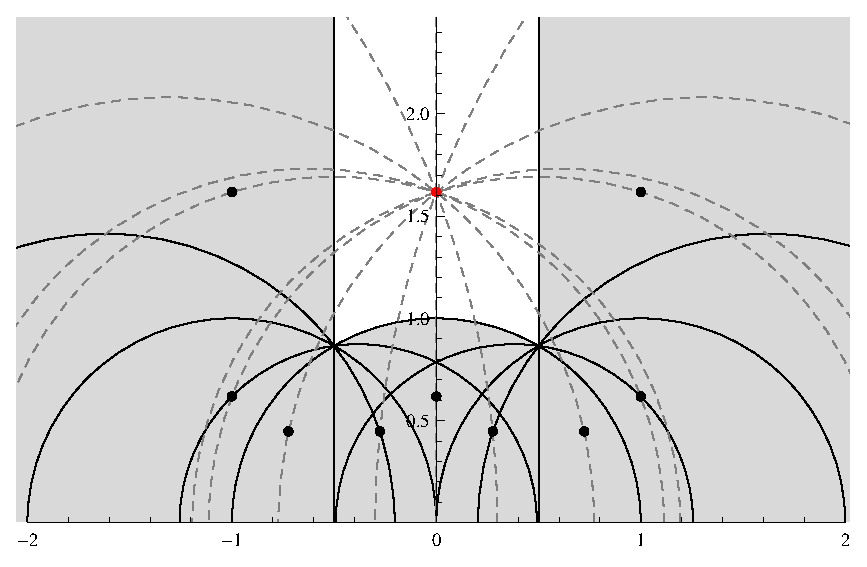
\includegraphics[width=.9\textwidth]{figures/normpoly-fundom-1}
\caption[The fundamental region $\FunDom$ as normal polygon]{The fundamental region $\FunDom$ can alternatively obtained by constructing the normal polygon with respect to a point $z$ on the imaginary axis with $\Im{z} > 1$. Above the point $z = \phi \ii$ (red) has been chosen, where $\phi = \frac{\sqrt{5}+1}{2}$ denotes the golden ratio.}
\label{fig_NormalPolyFunDom}
\end{figure}
\begin{figure}
\centering
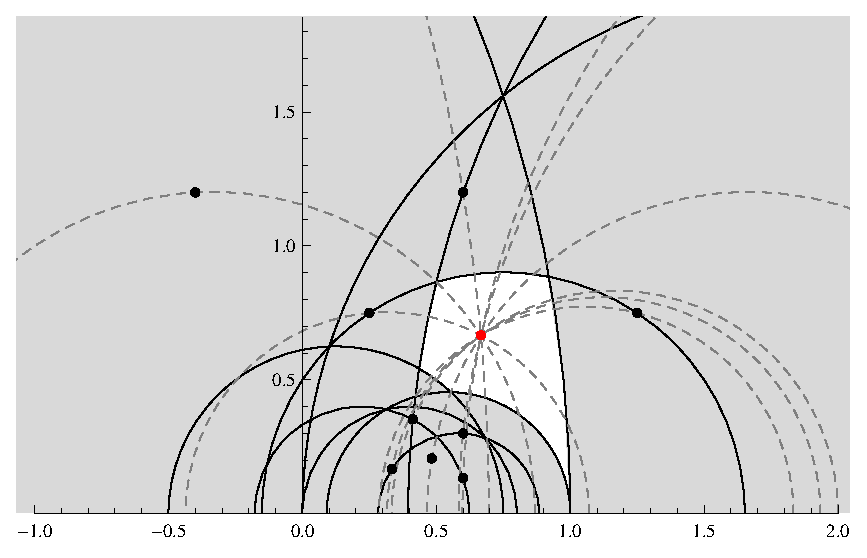
\includegraphics[width=.9\textwidth]{figures/normpoly-fundom-2}
\caption[An alternative fundamental region for $\PSL{\Z}$]{An alternative fundamental region for the action of $\PSL{\Z}$ on $\EU$. It is obtained by constructing the normal polygon for the point $\frac{2}{3}(1+\ii)$.}
\label{fig_AltNormalPolyFunDom}
\end{figure}

\begin{example}[Fundamental regions for $\PSL{\Z}$]
We see in Figure~\ref{fig_NormalPolyFunDom} that the fundamental region $\FunDom$ from (\ref{eqn_PSL2FunDom}) can alternatively be obtained by constructing the normal polygon for a point $z$ on the imaginary axis with $\Im{z} > 1$ (compare also Figure~\ref{fig_PSL2FunDom}). A different fundamental region for the action of $\PSL{\Z}$ on $\EU$ is displayed in Figure~\ref{fig_AltNormalPolyFunDom}.

In both figures, the point $z$ for which the normal polygon is constructed is colored red. Its equivalent points $Az$, $A \ne 1$ can be seen in black. For every pair $(z, Az)$, the corresponding perpendicular bisector (black) can be found best by following the gray dashed h-line which joins $Az$ with $z$.

Note that for producing an accurate picture of the normal polygon, it was in both cases sufficient to enumerate just 9 different transformations. In case of Figure~\ref{fig_NormalPolyFunDom}, all transformations with $n(A) \le 3$ have been selected, where $n(A)$ denotes the grading of $A$ as defined in (\ref{eqn_grading}). 

In Figure~\ref{fig_AltNormalPolyFunDom}, in order to achieve a good ``locality'' of the equivalent points $Az$ around $z$, additionally the fundamental set algorithm (Theorem~\ref{thm_FunSetAlg}) has been utilized: The selected transformations are all of the form $A = CB\inv{C}$ with $B \in \PSL{\Z}$, $n(B) \le 3$ and where $C$ denotes the transformation obtained when applying the fundamental set algorithm to $z$.
\end{example}

\begin{figure}
\centering
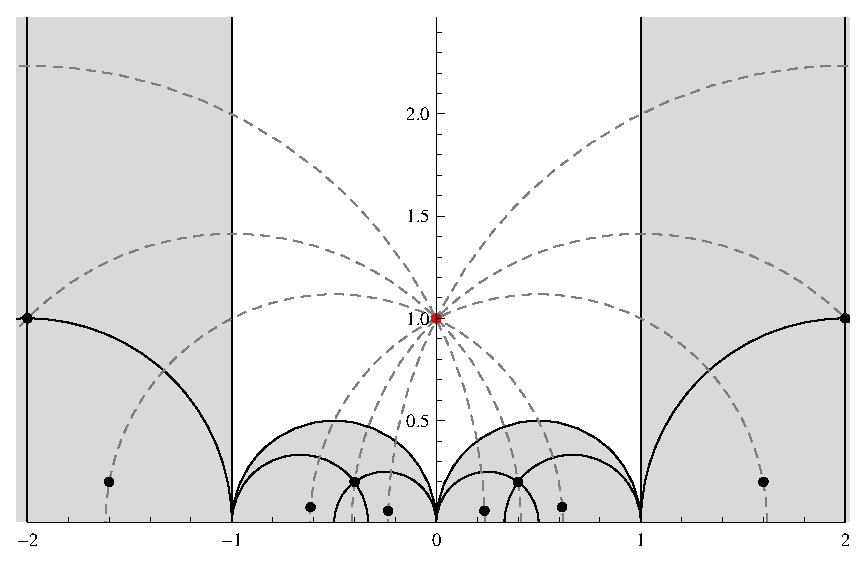
\includegraphics[width=.9\textwidth]{figures/normpoly-gamma2-1}
\caption[A fundamental region $\Gamma(2)$]{A fundamental region for the subgroup $\Gamma(2) \le \PSL{\Z}$. It is given by the normal polygon constructed with respect to the point $\ii$.}
\label{fig_Gamma2NormalPoly}
\end{figure}

\begin{example}
\index{Principal congruence subgroup}
As a demonstration of the normal polygon method in case of a proper subgroup of $\PSL{\Z}$, we see in Figure~\ref{fig_Gamma2NormalPoly} a normal polygon for the group $\Gamma(2) \le \PSL{\Z}$. For $m \in \N$, the \emph{principal congruence subgroup} $\Gamma(m)$ is defined as
\begin{equation*}
\Gamma(m) := \setdefsz{\bigg}{\mat{a}{b}{c}{d} \in \PSL{\Z}}{a \equiv d \equiv \pm 1,\ b \equiv c \equiv 0 \mod m}.
\end{equation*}
For drawing Figure~\ref{fig_Gamma2NormalPoly}, all nontrivial transformations in $\Gamma(2)$ with a grading not greater than $18$ (of which there are 12) have been selected. Note that for the particular chosen point $z$, also ``the first four'' nontrivial transformations of $\Gamma(2)$ (whose grading is $\le 6$) would have been enough to obtain the same region.
\end{example}
